%
% $RCSfile: knowledge_triumvirate.tex,v $
%
% Copyright (C) 2002-2008. Christian Heller.
%
% Permission is granted to copy, distribute and/or modify this document
% under the terms of the GNU Free Documentation License, Version 1.1 or
% any later version published by the Free Software Foundation; with no
% Invariant Sections, with no Front-Cover Texts and with no Back-Cover
% Texts. A copy of the license is included in the section entitled
% "GNU Free Documentation License".
%
% http://www.cybop.net
% - Cybernetics Oriented Programming -
%
% http://www.resmedicinae.org
% - Information in Medicine -
%
% Version: $Revision: 1.1 $ $Date: 2008-08-19 20:41:07 $ $Author: christian $
% Authors: Christian Heller <christian.heller@tuxtax.de>
%

\subsection{Knowledge Triumvirate}
\label{knowledge_triumvirate_heading}
\index{CYBOP Knowledge Triumvirate}
\index{Knowledge Triumvirate}
\index{Schema}
\index{Template}
\index{Model}
\index{CYBOP}
\index{CYBOL}
\index{CYBOI}
\index{Fourth Generation Languages}
\index{4GL}
\index{Object Oriented Programming Systems}
\index{OOPS}
\index{Computer Aided Software Engineering}
\index{CASE}
\index{Functional Programming}
\index{Procedural Language}
\index{Structured- and Procedural Programming}
\index{SPP}
\index{Side Effect}
\index{Knowledge Tree}
\index{State and Logic}
\index{Object Oriented Programming}
\index{OOP}
\index{Tree Structure}

Chapter \ref{knowledge_schema_heading} introduced a new \emph{Schema} for
knowledge representation; chapter \ref{cybernetics_oriented_language_heading}
defined a language for knowledge specification, in form of \emph{Templates};
chapter \ref{cybernetics_oriented_interpreter_heading} described a system for
knowledge processing, that uses \emph{Models}.

\begin{figure}[ht]
    \begin{center}
        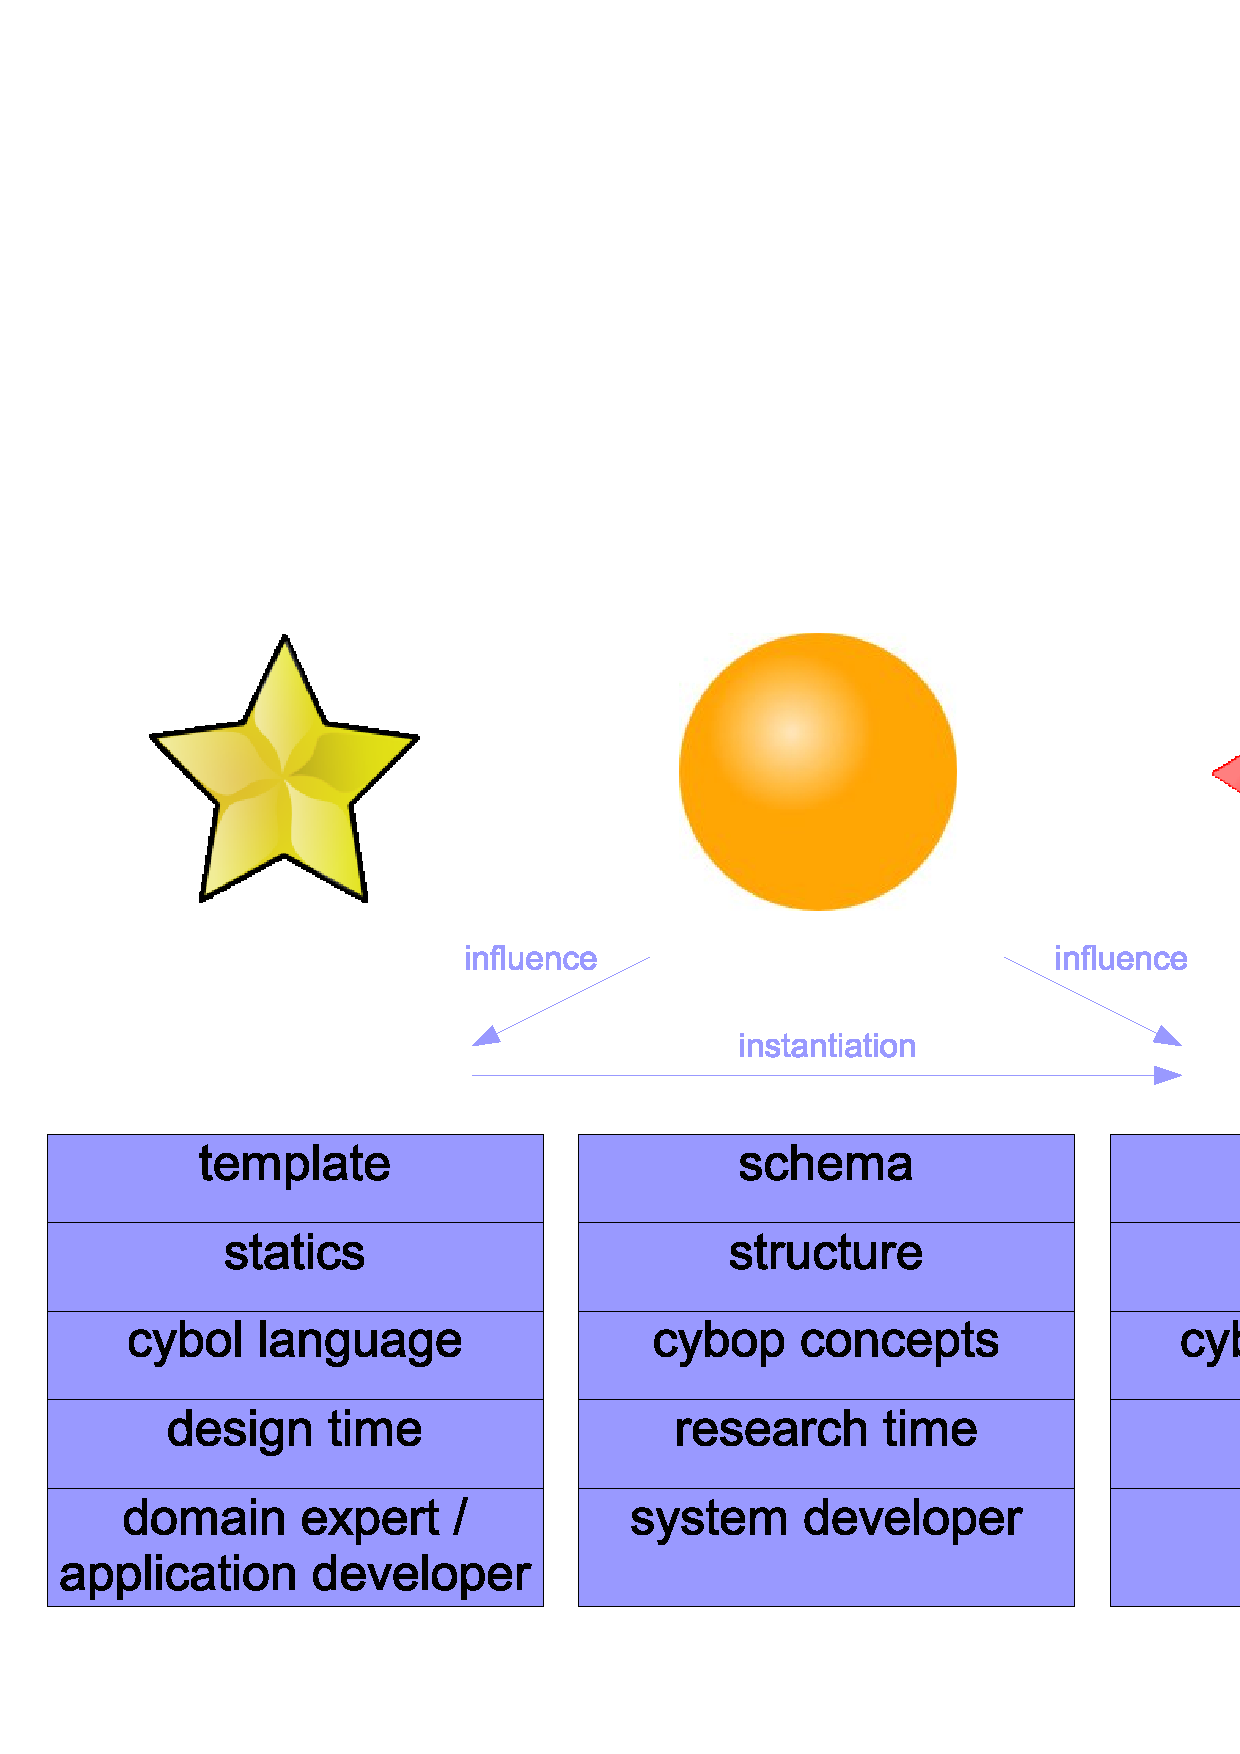
\includegraphics[scale=0.3,angle=-90]{graphic/triumvirate.pdf}
        \caption{Knowledge Triumvirate with Schema, Template and Model}
        \label{triumvirate_figure}
    \end{center}
\end{figure}

All three of them are closely connected (figure \ref{triumvirate_figure}): The
CYBOP knowledge \emph{Schema} provides a structure for both, knowledge
templates and -models; CYBOI \emph{Models} are the dynamic runtime instances of
static design-time CYBOL \emph{Templates}.

One reason for the mix-up of domain knowledge and system control in traditional
applications is the lack of a comprising solution for knowledge representation.
Software systems always have to fall back to using programming paradigms that
introduce more and more dependencies, as the system grows. John F. Sowa
\cite{sowa} writes:

\begin{quote}
    The enhanced productivity of the \emph{Fourth Generation Languages} (4GL),
    the \emph{Object Oriented Programming Systems} (OOPS) and the
    \emph{Computer Aided Software Engineering} (CASE) tools is derived from a
    common strength: improved methods of representing application knowledge in
    a form that can be used and reused by multiple system components. Their
    limitations result from a common weakness: the inability to share that
    knowledge with systems that use a different representation. The potential
    for conflict is inevitable: sharing requires a common representation, but
    independently developed systems almost invariably use different
    representations. In order to support knowledge sharing among heterogeneous
    systems, the conceptual schema must be general enough to accommodate anything
    that can be represented in any current system, any legacy system inherited
    from the past, and any new system that may be developed in the future.
\end{quote}

CYBOP claims to provide just that -- a common schema for knowledge
representation and -exchange. If not perfect, it is certainly a first step
towards an all-general knowledge schema.

Section \ref{functional_programming_heading} contained a quote in which the
\emph{Association of Lisp Users} \cite{commonlisp} states that, other than
\emph{Functional Programming}, \emph{Procedural Languages} essentially performed
everything as \emph{Side Effects} (variable updates persisting after expression
evaluation) to data structures. \textit{A purely procedural language}, after
\cite{commonlisp}, \textit{would have no functions, but might have subroutines
of no arguments that returned no values, and performed certain assignments and
other operations based on the data it found stored in the system.} This is
almost how CYBOI manipulates its knowledge -- in the manner of one huge side
effect. Its procedures do forward some parameters, but only one of these is
really application-related: the \emph{Knowledge Tree}. State- and logic
knowledge given in form of CYBOL templates are not bundled with low-level CYBOI
procedures. Both are configurable knowledge. Logic knowledge models do not get
input/ output (i/o) parameters handed over directly, but as dot-separated path
to the corresponding value in the knowledge tree.

Because all knowledge is stored in tree-form, application systems become much
more flexible than complex class networks as known from object-oriented
programming. Tree structures are easy to edit, with or without supportive tools.
They allow to better estimate necessary changes caused by new requirements,
because dependencies are obvious. Software maintenance gets improved, because
application developers can focus on pure domain knowledge; low-level system
functionality is provided by CYBOI. CYBOL applications are therefore absolutely
portable between platforms, as long as these were already considered in the
underlying CYBOI. Due to the straight-forward possibility of accessing parts of
a knowledge tree along well-defined paths, applications may win in performance.
